%%
%% This is file `ubcsample.tex',
%% generated with the docstrip utility.
%
% The original source files were:
%
% ubcthesis.dtx  (with options: `ubcsampletex')
%% 
%% This file was generated from the ubcthesis package.
%% --------------------------------------------------------------
%% 
%% Copyright (C) 2001
%% Michael McNeil Forbes
%% mforbes@alum.mit.edu
%% 
%% This file may be distributed and/or modified under the
%% conditions of the LaTeX Project Public License, either version 1.2
%% of this license or (at your option) any later version.
%% The latest version of this license is in
%%    http://www.latex-project.org/lppl.txt
%% and version 1.2 or later is part of all distributions of LaTeX
%% version 1999/12/01 or later.
%% 
%% This program is distributed in the hope that it will be useful,
%% but WITHOUT ANY WARRANTY; without even the implied warranty of
%% MERCHANTABILITY or FITNESS FOR A PARTICULAR PURPOSE.  See the
%% LaTeX Project Public License for more details.
%% 
%% This program consists of the files ubcthesis.dtx, ubcthesis.ins, and
%% the sample figures fig.eps and fig.fig.
%% 
%% This file may be modified and used as a base for your thesis without
%% including the licence agreement as long as the content (i.e. textual
%% body) of the file is completely rewritten. You must, however, change
%% the name of the file.
%% 
%% This file may only be distributed together with a copy of this
%% program. You may, however, distribute this program without generated
%% files such as this one.
%% 


% This Sample thesis requires \LaTeX2e
\NeedsTeXFormat{LaTeX2e}[1995/12/01]
%\ProvidesFile{ubcsample.tex}[2015/05/31 v1.72 ^^J
% University of British Columbia Sample Thesis]
% This is the \documentclass[]{} command.  The manditory argument
% specifies the "flavour" of thesis (ubcthesis for UBC).  The
% optional arguments (in []) specify options that affect how the
% thesis is displayed.  Please see the ubcthesis documentation for
% details about the options.
\documentclass[msc,oneside]{ubcthesis}
%\usepackage[pass,paperwidth=8.5in,paperheight=11in]{geometry}
\usepackage[
        paperwidth=8.5in,
        paperheight=11in,
        % other options: a3paper, a5paper, etc
        left=3.2cm,
        right=2.5cm,
        top=2.5cm,
        bottom=2.5cm,
        % use vmargin=2cm to make vertical margins equal to 2cm.
        % us  hmargin=3cm to make horizontal margins equal to 3cm.
        % use margin=3cm to make all margins  equal to 3cm.
        ]
{geometry}
%\pdfpageheight=11in
%\pdfpagewidth=8.5in
%
% To compile this sample thesis, issue the following commands:
% latex ubcsample
% bibtex ubcsample
% latex ubcsample
% latex ubcsample
% latex ubcsample
%
% To view use xdvi (on unix systems):
% xdvi ubcsample.dvi
%
% To make a postscript file, use dvips:
% dvips -o ubcsample.ps ubcsample.dvi
%
% To view the postscript file, use ghostview or gv (on unix systems):
% gv ubcsample.ps
%
%************************************************
% Optional packages.
%
% The use of these packages is optional, but they provide various
% tools for more flexible formating.  The sample thesis uses these,
% but if you remove the example code, you should be able to exclude
% these packages.  Only standard packages have been described here;
% they should be installed with any complete LaTeX instalation, but
% if not, you can find them at the Comprehensive TeX Archive Network
% (CTAN): http://www.ctan.org/
%

%******** afterpage ***************************
% This package allows you to issue commands at the end of the current
% page.  A good use for this is to use the command
% \afterpage{\clearpage} right after a figure.  This will cause the
% figure to be inserted on the page following the current one (or on
% the current page if it will fit) but will not break the page in the
% middle.
\usepackage{afterpage}
\usepackage{xcolor}
%******** float *********************************
% This package allows you to customize the style of
% "floats"---floating objects such as figures and tables.  In
% addition, it allows you to define additional floating objects which
% may be included in a list similar to that produces by \listoftables
% and \listoffigures.  Common uses include introducing floats for
% programs and other code bits in Compute Science and Chemical Schema.
\usepackage{float}
\usepackage{amsmath,bm}
%******** tocloft *******************************
% This package allows you to customize and define custom lists such
% as a list of programs or Chemical Scheme.  Note: if you use the
% subfigure package, you must specify that you do as an option here.
% The title option uses the default formatting.  We do not use this
% here as the default formatting is acceptable.  Use the float
% package instead unless you need the extra formatting control
% provided by tocloft.
%\usepackage[subfigure, titles]{tocloft}

%******** alltt *********************************
% The alltt package allows you to include files and have them
% formatted in a verbatim fashion.  This is useful for including
% source code from an additional file.
%\usepackage{alltt}

%******** listings ******************************
% The listings package may be used to include chunks of source code
% and has facilities for pretty-printing many languages.
%\usepackage{listings}

%******** longtable *****************************
% The longtable package allows you to define tables that span
% multiple pages.



\usepackage{longtable}

%******** graphics and graphicx *****************
% This allows you to include encapsulated postscript files.  If you
% don't have this, comment the \includegraphics{} line following the
% comment "%includegraphics" later in this file.
\usepackage{graphicx}

%******** subfigure *****************************
% The subfigure package allows you to include multiple figures and
% captions within a single figure environment.
%\usepackage{subfigure}

%******** here **********************************
% The here package gives you more control over the placement of
% figures and tables.  In particular, you can specify the placement
% "H" which means "Put the figure here" rather than [h] which means
% "I would suggest that you put the figure here if you think it looks
% good."
%\usepackage{here}

%******** pdflscape ********************************
% This allows you to include landscape layout pages by using the
% |landscape| environment.  The use of |pdflscape| is preferred over
% the standard |lscape| package because it automatically rotates the
% page in the pdf file for easier reading.  (Thanks to Joseph Shea
% for pointing this out.)
\usepackage{pdflscape}

%******** natbib ********************************
% This is a very nice package for bibliographies.  It includes options
% for sorting and compressing bibliographic entries.
\usepackage[numbers,sort&compress]{natbib}
%\usepackage{natbib}   % omit 'round' option if you prefer square brackets

%\usepackage{hyperref}
\usepackage[unicode=true,
  colorlinks=true,
  linktocpage,
  linkbordercolor={0.5 0.5 1},
  citebordercolor={0.5 1 0.5},
  linkcolor=blue]{hyperref}


\usepackage[nameinlink]{cleveref}


% for clever referencing, i.e. references equations as e.g.: eq. (1.1), particularly useful together with hyperref (which is automatically loaded by jcappub)

%******** psfrag ******************************
% This allows you to replace text in postscript pictures with formated
% latex text.  This allows you to use math in graph labels
% etc. Uncomment the psfrag lines following the "%psfrag" comment
% later in this file if you don't have this package.  The replacements
% will only be visible in the final postscript file: they will be
% listed in the .dvi file but not performed.
%\usepackage{psfrag}
%\usepackage[margin=0.5in]{geometry}
%******** hyperref *****************************
% Please read the manual:
% http://www.tug.org/applications/hyperref/manual.html
%
% This adds hyperlinks to your document: with the right viewers (later
% versions of xdvi, acrobat with pdftex, latex2html etc.) this will
% make your equation, figure, citation references etc. hyperlinks so
% that you can click on them.  Also, your table of contents will be
% able to take you to the appropriate sections.  In the viewers that
% support this, the links often appear with an underscore.  This
% underscore will not appear in printed versions.
%
% Note: if you do not use the hypertex option, then the dvips driver
% may be loaded by default.  This will cause the entries in the list
% of figures and list of tables to be on a single line because dvips
% does not deal with hyperlinks on broken lines properly.
%
% NOTE: HYPERREF is sensitive to the ORDER in which it is LOADED.
% For example, it must be loaded AFTER natbib but BEFORE newly
% defined float environments.  See the README file with the hyperref
% for some help with this.  If you have some very obscure errors, try
% first disabling hyperref.  If that fixes the problem, try various
% orderings.
%
% Note also that there is a bug with versions before 2003/11/30
% v6.74m that cause the float package to not function correctly.
% Please ensure you have a current version of this package.  A
% warning will be issued if you leave the date below but do not have
% a current version installed.
%
% Some notes on options: depending on how you build your files, you
% may need to choose the appropriate option (such as [pdftex]) for the
% backend driver (see the hyperref manual for a complete list).  Also,
% the default here is to make links from the page numbers in the table
% of contents and lists of figures etc.  There are other options:
% excluding the [linktocpage] option will make the entire text a
% hyperref, but for some backends will prevent the text from wrapping
% which can look terrible.  There is a [breaklinks=true] option that
% will be set if the backend supports (dvipdfm for example supports
% it but does not work with psfrag.)
%
% Finally, there are many options for choosing the colours of the
% links.  These will be included by default in future versions but
% you should probably consider changing some now for the electronic
% version of your thesis.
%\usepackage[unicode=true,
%  linktocpage,
%  linkbordercolor={0.5 0.5 1},
%  citebordercolor={0.5 1 0.5},
%  linkcolor=blue]{hyperref}

% If you would like to compile this sample thesis without the
% hyperref package, then you will need to comment out the previous
% \usepackage command and uncomment the following command which will
% put the URL's in a typewriter font but not link them.
%\newcommand\url[1]{\texttt{#1}}

%******** setspace *******************************
% The setspace package allows you to manually set the spacing of the
% file.  UBC may require 1.5 spacing for microfilming of theses.  In
% this case you may obtain this by including this package and issuing
% one of the following commands:
%\usepackage{setspace}
%\singlespacing
%\onehalfspacing
%\doublespacing

% These commands are optional.  The defaults are shown.  You only
% need to include them if you need a different value
\institution{The University Of British Columbia}

% If you are at the Okanagan campus, then you should specify these
% instead.
%\faculty{The College of Graduate Studies}
%\institutionaddress{Okanagan}
\faculty{The Faculty of Graduate and Postdoctoral Studies}
\institutionaddress{Vancouver}

% You can issue as many of these as you have...
\previousdegree{B.Sc., University of British Columbia, year}
%\previousdegree{M.Sc., The University of British Columbia, 2022}
%\previousdegree{Ph.D., Massachusetts Institute of Technology, 2005}

% You can override the option setting here.
% \degreetitle{Jack of All Trades}

% These commands are required.
\title{Title}
%\subtitle{With a Subtitle}
\author{Author}
%\copyrightyear{2000}
\submitdate{\monthname\ \number\year} % The "\ " is required after
                                      % \monthname to prevent the
                                      % command from eating the space.
\program{program}

% These commands are presently not required for UBC theses as the
% advisor's name and title are not presently required anywhere.
%\advisor{Ariel R.~Zhitnitsky}
%\advisortitle{Professor of Physics}

% One might want to override the format of the section and chapter
% numbers.  This shows you how to do it.  Note that the current
% format is acceptable for submission to the FoGS: If you wish to modify
% these, you should check with the FoGS explicity. prior to making
% the modifications.
\renewcommand\thepart         {\Roman{part}}
\renewcommand\thechapter      {\arabic{chapter}}
\renewcommand\thesection      {\thechapter.\arabic{section}}
\renewcommand\thesubsection   {\thesection.\arabic{subsection}}
\renewcommand\thesubsubsection{\thesubsection.\arabic{subsubsection}}
\renewcommand\theparagraph    {\thesubsubsection.\arabic{paragraph}}
\renewcommand\thesubparagraph {\theparagraph.\arabic{subparagraph}}

\setcounter{tocdepth}{2}
\setcounter{secnumdepth}{2}
%\newcommand{\arefe}[1]{{\textcolor{cyan}{#1}}}
% Here is an example of a "Program" environment defined with the
% "float" package.  The list of programs will be stored in the file
% ubcsample.lop and the numbering will start with the chapter
% number.  The style will be "ruled".
\floatstyle{ruled}
\newfloat{Program}{htbp}{lop}[chapter]

% Here is the start of the document.
\begin{document}

%% This starts numbering in Roman numerals as required for the thesis
%% style and is mandatory.
\frontmatter

%%% The order of the following components should be preserved.  The order
%%% listed here is the order currently required by FoGS:        \\
%%% Title (Mandatory)                                           \\
%%% Preface (Manditory if any collaborator contributions)       \\
%%% Abstract (Mandatory)                                        \\
%%% List of Contents, Tables, Figures, etc. (As appropriate)    \\
%%% Acknowledgements (Optional)                                 \\
%%% Dedication (Optional)                                       \\

\maketitle                      %% Mandatory

\clearpage

%%%THESIS APPROVAL PAGE - REQUIRED AS PART OF YOUR COMPLETED THESIS

%%%%%%% UBC FoGPS Requires the following statements at the beginning of the thesis. There is a (separate) thesis approval form that has to be signed and dated by the same individuals listed here as approving the thesis. You will have to get ensure that your department submits that approval form before you will be able to create an account and upload your thesis onto ciRCle. 
\noindent
The following individuals certify that they have read, and recommend to the Faculty of Graduate and Postdoctoral Studies for acceptance, the thesis entitled:

\bigskip\noindent
\textbf{Title}



\bigskip\noindent
submitted by 
\textbf{Author}
in partial fulfillment of the requirements for
the degree of 
\textbf{program}
\bigskip\noindent
in	\textbf{Physics}


\bigskip\noindent
%\textbf{[Include titles, departments, and universities, or titles and organizations. Remember to remove ALL material in square brackets [  ] before adding the page to your thesis.] Modify the examining committee to adapt to your case.}

\bigskip\noindent
\textbf{Examining Committee:}

\bigskip\noindent
Supervisor: 

%\bigskip\noindent
%Co-supervisor: \hrulefill

%\bigskip\noindent
%Supervisory Committee Member: \hrulefill

\bigskip\noindent
Additional Examiner: 

%\bigskip\noindent
%Additional Supervisory Committee Members: 

%\bigskip\noindent
%Supervisory Committee Member:\hrulefill







\clearpage
\begin{abstract}                %% Mandatory -  maximum 350 words
  The \texttt{genthesis.cls} \LaTeX{} class file and accompanying
  documents, such as this sample thesis, are distributed in the hope
  that it will be useful but without any warranty (without even the
  implied warranty of fitness for a particular purpose).  For a
  description of this file's purpose, and instructions on its use, see
  below.

\end{abstract}

\chapter{Lay Summary}

%[Required, Maximum 150 words]

%This is a simple summary of your thesis, written so that members of the public will get some idea about what you have done.

%Full-sky simulations of the foreground radiation of the cosmic microwave background are computationally expensive and it is challenging to measure if they can replicate the same statistical properties as the real data. 
%In this thesis, I advocate for the use of a method called the ``hierarchical wavelet coefficients" for characterizing non-Gaussianities in a spherical field. This method is also known as the ``wavelet scattering transform" method and so far it has been mostly used for analysing flat (cutsky) maps. I demonstrate that the full-sky implementation introduced in this thesis is also capable of characterizing non-Gaussianities using a small set of coefficients.  

%The algorithm for this method is based on the  \textsc{Healpy} package. 

%I demonstrate that we can check the non-Gaussianity in simulated maps. I propose that this method can potentially serve as a tool for measuring and controlling the amount of non-Gaussianity in future simulations. 
[Required, Maximum 150 words]

This is a simple summary of your thesis, written so that members of the public will get some idea about what you have done. 

\chapter{Preface}
% Manditory if any of the conditions are met

You must include a preface if any part of your research was partly or
wholly published in articles, was part of a collaboration, or required
the approval of UBC Research Ethics Boards.

The Preface must include the following:

\begin{itemize}
\item A statement indicating the relative contributions of all
  collaborators and co-authors of publications (if any), emphasizing
  details of your contribution, and stating the proportion of research
  and writing conducted by you.
\item A list of any publications arising from work presented in the
  dissertation, and the chapter(s) in which the work is located.
\item The name of the particular UBC Research Ethics Board, and the
  Certificate Number(s) of the Ethics Certificate(s) obtained, if
  ethics approval was required for the research.
\end{itemize}

Thats's what I wrote:

The content of this thesis is original unpublished work by the author. The idea for this study came about through discussions with author's supervisor, Dr. supervisor. All necessary python scripts, as well as the resulting plots and data were created by the author. Individual techniques and methods used but not developed by the author have been cited where appropriate.


\tableofcontents %% Mandatory
\listoftables                   %% Mandatory if thesis has tables
\listoffigures                  %% Mandatory if thesis has figures
%\listof{Program}{List of Programs} %% Optional
%% Any other lists should come here, i.e.
%% Abbreviation schemes, definitions, lists of formulae, list of
%% schemes, glossary, list of symbols etc.

\chapter{Acknowledgements}      %% Optional
This is the place to thank professional colleagues and people who have
given you the most help during the course of your graduate work.


%\chapter{Dedication} %% Optional
%The dedication is usually quite short, and is a personal rather than
%an academic recognition.  The \emph{Dedication} does not have to be
%titled, but it must appear in the table of contents.  If you want to
%skip the chapter title but still enter it into the Table of Contents,
%use this command \verb|\chapter[Dedication]{}|.

%Note that this section is the last of the preliminary pages (with
%lowercase Roman numeral page numbers).  It must be placed
%\emph{before} the \verb|\mainmatter| command.  After that, Arabic
%numbered pages will begin.

% Any other unusual prefactory material should come here before the
% main body.

% Now regular page numbering begins.
\mainmatter

% Parts are the largest structural units, but are optional.
%\part{Thesis}

% Chapters are the next main unit.
%\chapter{Contents}
%\begin{enumerate}
    \item Introduction
\begin{itemize}
    \item The standard model of cosmology
    \item what is non-Gaussianity
    \item non-Gaussianity in cosmology and astrophysics
\end{itemize}
\item Wavelet Scattering Transform
\begin{itemize}
    \item previous studies done
    \item what is ST
    \item what are its features 
    \item what is wavelet 
    \item Morlet wavelet in flat space 
    \item How do we define morlet wavelet in curved space 
    \item are our curved morlets actually wavelets?
    \item how do we normalize them 
\end{itemize}
\item Results 
\begin{itemize}
    \item sz: what is sz?
    \item sz is non-Gaussian 
    \item first order coeffs 
    \item second order coeffs 
    \item masked maps
    \item simulated or fake maps?
    \item foreground 
    \item results of foreground  
    \item pysm-generated maps
\end{itemize}
\item Future
\begin{itemize}
    \item parameter estimatioin 
    \item simulating?
\end{itemize}
\end{enumerate}





\chapter{Introduction}
\section{section1}

babble babble babble babble babble babble babble babble babble babble

\section{section2}
babble babble babble babble babble babble babble babble babble babble
\begin{figure}[h!]
    \centering
    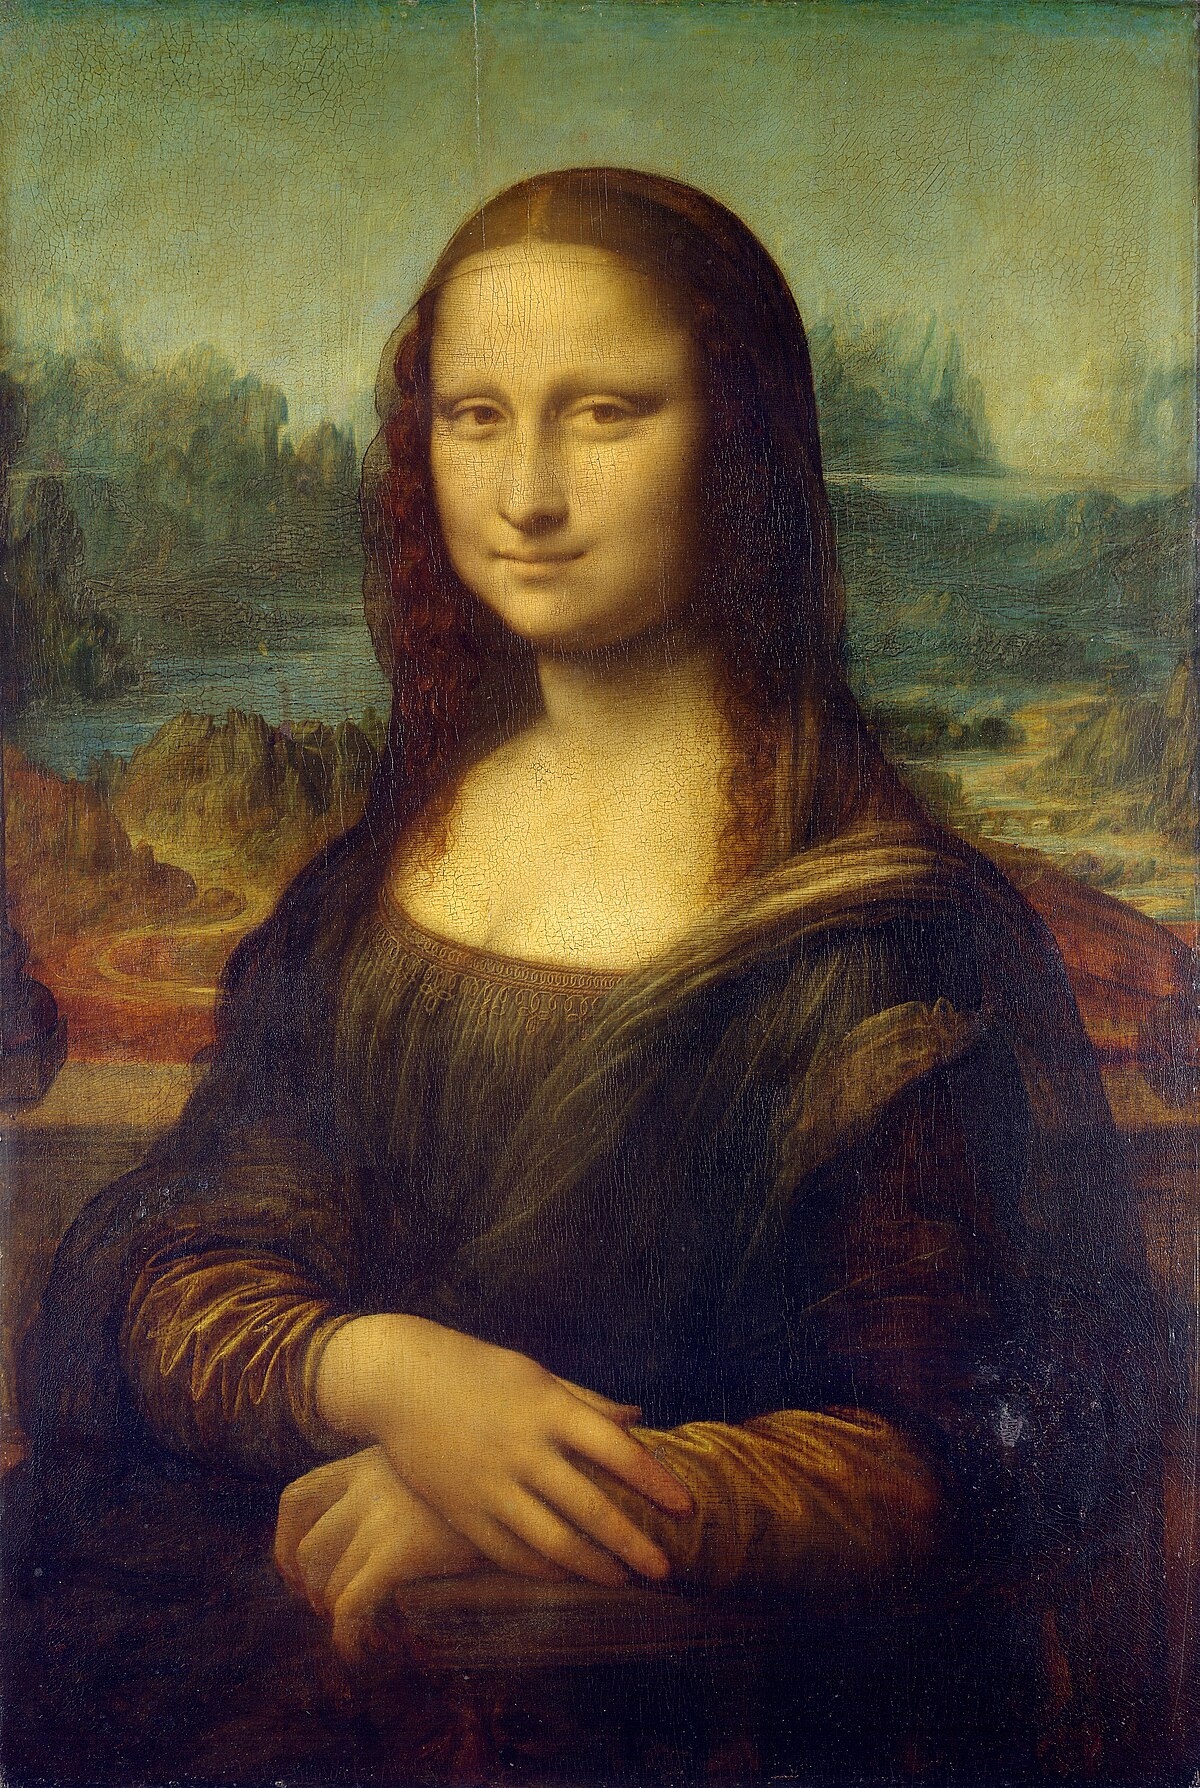
\includegraphics[width=0.5\linewidth]{Figures/Mona_Lisa.jpg}
    \caption{caption}
    \label{fig:illustris}
\end{figure}

\begin{equation}
  \mathrm{f}(x)=\int_{-\infty}^{\int_{-\infty}^x
    e^{-\frac{y^2}{2}}\mathrm{d}{y}}e^{-z^2}\mathrm{d}z
\end{equation}

\chapter{Thesis}
\begin{Program}
  \caption{\label{prog:fib} Python program that computes the $n^{\rm
      th}$ Fibonacci number using memoization.}
\begin{verbatim}
def fib(n,_cache={}):
    if n < 2:
        return 1
    if n in _cache:
        return _cache[n]
    else:
        result = fib(n-1)+fib(n-2)
        _cache[n] = result
        return result
\end{verbatim}
\end{Program}

In~\cite{1929PNAS...15..168H} they say ~\cite{1948MNRAS.108..252B}

\chapter{Results}
\section{Tables}
We have already included one table:~\ref{tab:Table1}.  Another table
is plopped right here.
\begin{table}[ht]
  \begin{center}
    \begin{tabular}{|l||l|l||l|l|}
      \hline
      &\multicolumn{2}{l|}{Singular}&\multicolumn{2}{l|}{Plural}\\
      \cline{2-5}
       &English&\textbf{Gaeilge}&English&\textbf{Gaeilge}\\
      \hline\hline
      1st Person&at me&\textbf{agam}&at us&\textbf{againn}\\
      2nd Person&at you&\textbf{agat}&at you&\textbf{agaibh}\\
      3rd Person&at him&\textbf{aige}&at them&\textbf{acu}\\
       &at her&\textbf{aici}& & \\
      \hline
    \end{tabular}
    \caption{
      \label{tab:Table2}
      Another table.}
  \end{center}
\end{table}
\input{Results/RSLT02}
\chapter{Discussion}
discussion 


%% This file is setup to use a bibtex file sample.bib and uses the
%% plain style.  Other styles may be used depending on the conventions
%% of your field of study.
%%
%%% Note: the bibliography must come before the appendices.
% \bibliographystyle{JHEP}
% \bibliographystyle{plainnat}
\bibliographystyle{unsrt}
\bibliography{references,refs}
%\printbibliography  %[heading=none, keyword=OWN]
%% Use this to reset the appendix counter.  Note that the FoGS
%% requires that the word ``Appendices'' appear in the table of
%% contents either before each appendix lable or as a division
%% denoting the start of the appendices.  We take the latter option
%% here.  This is ensured by making the \texttt{appendicestoc} option
%% a default option to the UBC thesis class.

%%% If you only have one appendix, please uncomment the following line.
% \renewcommand{\appendicesname}{Appendix}
\appendix
\chapter{First Appendix}
%In this appendix, I show that the spherical Morlet wavelet introduced in \cref{sec:ST} satisfies all wavelet requirements. 
There are three conditions for a wavelet:

\begin{enumerate}
    \item translation invariant 
    \item localized in both real space and Fourier space 
    \item wavelet should be admissible 
    \begin{equation}
        c_{\psi} \equiv (2 \pi)^2 \int_{\mathbb{R}^2} \frac{|\widetilde{\psi}(k)|^{2}}{|k|^2} d k<\infty
    \end{equation}
        which essentially gives a weaker admissibility condition
        \begin{equation}
            \widetilde{\psi}(0) = 0
        \end{equation}

    
\end{enumerate}

%\chapter{Second Appendix}
%Here is the second appendix.

%% This changes the headings and chapter titles (no numbers for
%% example).
\backmatter

%% Indices come here if you have them.








    %\url{http://www.grad.ubc.ca/current-students/dissertation-thesis-preparation}\\
   

\end{document}
\endinput
%%
%% End of file `ubcsample.tex'.
